\chapter{Flujo Compresible}

	
	En las sesiones introductorias del curso vimos que el criterio de
	compresibilidad relacionaba la presión con la velocidad del flujo.
	Para el aire la velocidad a partir de la cual el flujo puede y debe
	ser considerado compresible está alrededor de $40~\text{m/s}$. Teóricamente
	también los líquidos en ciertas condiciones pueden ser considerados
	compresibles. Pero estas condiciones son dificiles de conseguir en
	la práctica (unos $200~\text{m/s}$ y/o más de $200~\text{atm}$).
	
	En el estudio de flujo compresible tiene un papel importante la termodinámica
	del proceso.
	
	El parámetro más importante en el estudio del flujo compresible es
	el número de Mach, 
	
\begin{equation}
		\ma=\frac{u}{c}
\end{equation}
	
	donde $c$ es la velocidad del sonido es el fluido, que depende,
	como veremos de la temperatura del fluido.


\section{Repaso de Termodinámica}

	
	La variación de entropí a se calcula a partir de las dos primeras
	leyes de la Termodinámica, que, para un gas perfecto, da 
	
\begin{equation}
		T\dif s=\dif h-\frac{\dif p}{\rho}=c_{p}\dif T-\frac{\dif p}{\rho}
\end{equation}
	
	
	Dado que 
	\[
	\frac{p}{\rho}=rT\,;\,\text{con }r=\frac{R}{M}=c_{p}-c_{v},
	\]
	
	\[
	\dif s=c_{p}\frac{\dif T}{T}-r\frac{\dif p}{p}
	\]
	
	\[
	\Rightarrow\,\int_{1}^{2}\dif s=\int_{1}^{2}c_{p}\frac{\dif T}{T}-r\ln\frac{p_{2}}{p_{1}}
	\]
	
	
	Si $c_{p}$ es variable, la integral se resuelve de forma numérica
	o con la ayuda de tablas. Si puede ser considerada constante, 
	
\begin{equation}
		s_{2}-s_{1}=c_{p}\ln\frac{T_{2}}{T_{1}}-r\ln\frac{p_{2}}{p_{1}}
\end{equation}
	
	
	Si realizamos el mismo cálculo, pero a partir de $\dif s=c_{v}\dif T-p\dif\frac{1}{\rho}$
	habríamos llegado a 
	
\begin{equation}
		s_{2}-s_{1}=c_{v}\ln\frac{T_{2}}{T_{1}}-r\ln\frac{\rho_{2}}{\rho_{1}}
\end{equation}
	
	
	Estas relaciones nos permiten calcular la variación de entropía en
	procesos no isoentrópicos, como puede ser, por ejemplo el frente de
	una onda de choque.
	
	Si el proceso es isoentrópico, $s_{2}-s_{1}=0$ y podemos escribir
	las conocidas relaciones 
	
\begin{equation}
		\frac{p_{2}}{p_{1}}=\left(\frac{\rho_{2}}{\rho_{1}}\right)^{\gamma}=\left(\frac{T_{2}}{T_{1}}\right)^{\frac{\gamma}{\gamma-1}}\;\text{con }\;\gamma=\frac{c_{p}}{c_{v}}
\end{equation}
	
	

\section{La velocidad del sonido}

	
	El sonido no es más que una onda de presión de amplitud pequeña.
	
	\medskip{}
	
	\begin{tabular}{cc}
		\begin{minipage}[c]{0.3\textwidth}%
			\begin{center}
				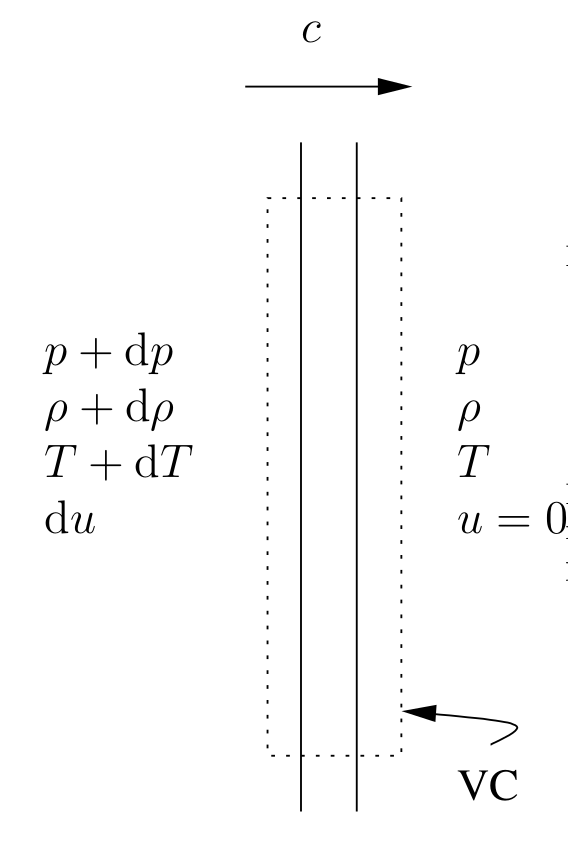
\includegraphics[width=\linewidth]{TeX_files/chapter11-Compresible/onda1}
			\end{center}
		
		\end{minipage} & %
		\begin{minipage}[c]{0.6\textwidth}%
			Por continuidad, 
			\[
			\int_{SC}\rho\vec{u}_{r}\cdot\dif\vec{S}=-\rho cA+(\rho+\Delta\rho)(c-\Delta u)A=0
			\]
			
			\[
			\Rightarrow\,\Delta u=c\,\frac{\Delta\rho}{\rho+\Delta\rho}
			\]
			
			Dado que no hay gradiente de velocidad en la dirección normal al flujo,
			no hay fricción, y la conservación de la cantidad de movimiento nos
			permite relacionar la velocidad de la onda con la variación de presión %
		\end{minipage}\tabularnewline
	\end{tabular}

	
	\[
	-\Delta pA=\dot{m}(u_{2}-u_{1})=\rho Ac(-\Delta u)\,\Rightarrow\,\Delta p=\rho c\Delta u
	\]
	
	\[
	\Delta p=\rho c\left[c\,\frac{\Delta\rho}{\rho+\Delta\rho}\right]=c^{2}\,\frac{\rho\Delta\rho}{\rho+\Delta\rho}
	\]
	
	\[
	\Rightarrow c^{2}=\frac{\Delta p}{\Delta\rho}\left[1+\frac{\Delta\rho}{\rho}\right]
	\]
	
	En el límite $\Delta\rho\rightarrow0$, hablamos de velocidad del
	sonido, 
	
\begin{equation}
		\boxed{c=\sqrt{\dparc{p}{\rho}}}
\end{equation}
	
	
	
	Si el proceso es adiabático (no hay gradientes de temperatura en el interior
	o exterior de la onda) 
	\[
	c=\sqrt{\left.\dparc{p}{\rho}\right|_{s}}=\sqrt{\gamma\left.\dparc{p}{\rho}\right|_{T}}
	\]
	
	Para un gas perfecto, $\left.\dparc{p}{\rho}\right|_{T}=rT$, de forma
	que 
	\[
	c=\sqrt{\gamma rT}
	\]
	
	Para el aire, $\gamma=1.4$ y $r=287$, de forma que 
	\[
	c\approx20\sqrt{T}
	\]
	con $T$ en Kelvins y $c$ en m/s. A $20^{\circ}\,C$, $c\approx340\,\text{m/s}\approx1220\,\text{km/h}$


\section{Flujo adiabático}

	
	Ecuación de Bernoulli (la poca densidad del fluido hace que el término
	de gravedad sea menospreciable) 
	
\begin{equation}
		h+\frac{u^{2}}{2}=\text{cte}=h_{0}
\end{equation}
	
	
	$h_{0}$ : \textcolor{red}{entalpía de estancamiento}. Entalpía que
	obtendríamos en el fluido si lo llevásemos al reposo de forma adiabática.
	
	Para gases reales, el cálculo de la entalpía para una cierta temperatura
	debe realizarse con tablas. Para gases perfectos, $h=c_{p}T$, 
	
\begin{equation}
		c_{p}T+\frac{u^{2}}{2}=c_{p}T_{0}
\end{equation}
	
	
	$T_{0}$ : Temperatura de estancamiento
	
	Si la entalpía (o la temperatura) son llevados a cero de forma adiabática,
	la velocidad del flujo alcanza su valor máximo, 
	\[
	u_{max}=\sqrt{2h_{0}}
	\]
	
	\[
	u_{max}=\sqrt{2c_{p}T_{0}}\qquad\text{para un gas perfecto}
	\]
	
	Podemos obtener la \textcolor{blue}{forma adimensional de la ecuación
		de Bernoulli}, 
	
\begin{equation}
		1+\frac{u^{2}}{2c_{p}T}=\frac{T_{0}}{T}
\end{equation}
	
	o bien, usando $c_{p}T=\gamma rT/(\gamma-1)=c^{2}/(\gamma-1)$, 
	
\begin{equation}
		\boxed{1+\frac{\gamma-1}{2}\ma^{2}=\frac{T_{0}}{T}}
\end{equation}
		
	Dado que la velocidad del sonido es proporcional a $\sqrt{T}$, 
	
\begin{equation}
		\frac{c_{0}}{c}=\sqrt{\frac{T_{0}}{T}}=\left[1+\frac{\gamma-1}{2}\ma^{2}\right]^{1/2}
\end{equation}
	
	
	Estas expresiones son válidas siempre que el flujo sea adiabático.
	Si, además, es isoentrópico (es decir, reversible), para un gas perfecto
	tenemos 
	\begin{eqnarray}
		\frac{p_{0}}{p}=\left(\frac{T_{0}}{T}\right)^{\frac{\gamma}{\gamma-1}}=\left[1+\frac{\gamma-1}{2}\ma^{2}\right]^{\frac{\gamma}{\gamma-1}}\\
		\frac{\rho_{0}}{\rho}=\left(\frac{T_{0}}{T}\right)^{\frac{1}{\gamma-1}}=\left[1+\frac{\gamma-1}{2}\ma^{2}\right]^{\frac{1}{\gamma-1}}
	\end{eqnarray}
	


\section{Valores sónicos}
	
	Además de $T_{0}$, $p_{0}$, $\rho_{0}$ y $c_{0}$, también son
	útiles los valores denominados \textcolor{red}{sónicos}, o \textcolor{red}{críticos}, obtenidos cuando $\ma=1.0$,
	
	 $p^{*}=p_{0}\left(\frac{2}{\gamma+1}\right)^{\frac{\gamma}{\gamma-1}};T^{*}=T_{0}\frac{2}{\gamma+1};\rho^{*}=\rho_{0}\left(\frac{2}{\gamma+1}\right)^{\frac{1}{\gamma-1}};c^{*}=c_{0}\left(\frac{2}{\gamma+1}\right)^{\frac{1}{2}}(=u^{*})$


	
	\textbf{Ejemplo :}
		\begin{tabular}{cc}
			\begin{minipage}[c]{0.5\textwidth}%
\begin{center}
	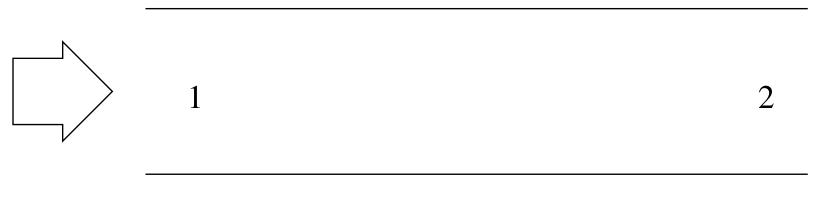
\includegraphics[width=1\linewidth]{TeX_files/chapter11-Compresible/ejemplo1}
\end{center}
Flujo adiabático de aire
			\end{minipage} & %
			\begin{minipage}[c]{0.4\textwidth}%
				
				\begin{eqnarray*}
					u_{1} & = & 240\,\text{m/s}\\
					T_{1} & = & 320\,\text{K}\\
					p_{1} & = & 170\,\text{kPa}
				\end{eqnarray*}
				%
			\end{minipage}\tabularnewline
		\end{tabular}

\bigskip
		
		Queremos calcular ${T_{0}}_{1}$, ${p_{0}}_{1}$, ${\rho_{0}}_{1}$,
		$\ma_{1}$, ${u_{max}}_{1}$ y $u_{1}^{*}$.
		
		Si $u_{2}=290\,\text{m/s}$ y $p_{2}=135\,\text{kPa}$, calcular ${p_{0}}_{2}$.
		
		Dado que no sabemos si el flujo es isoentrópico o no, sólo podemos
		usar las relaciones isoentrópicas para calcular $p_{0}$ y $\rho_{0}$
		de forma local en 1. {\footnotesize{}
			\begin{eqnarray*}
				r & = & 287\,\text{J/Kg\, K}\\
				\gamma & = & 1.4\\
				c_{p} & = & 1005\,\text{J/Kg\, K}
			\end{eqnarray*}
		}{\footnotesize\par}

		\begin{tabular}{c|c}
			\begin{minipage}[c]{0.45\textwidth}%
				Empezamos calculando Ma, {\footnotesize{}
					\[
					c_{1}=\sqrt{\gamma rT_{1}}=358.6\,\text{m/s}
					\]
					\[
					\Rightarrow\,\ma_{1}=\frac{240}{358.6}=0.67
					\]
					\[
					{T_{0}}_{1}=\left[1+\frac{\gamma-1}{2}\ma^{2}\right]T_{1}=348.7\,\text{K}
					\]
				}{\footnotesize\par}
				
				Otra forma de calcularlo habría sido con 
				\[
				{T_{0}}_{1}=T_{1}+\frac{u_{1}^{2}}{2c_{p}}
				\]
				%
			\end{minipage} & %
			\begin{minipage}[c]{0.45\textwidth}%
				{\footnotesize{}
					\begin{eqnarray*}
						{p_{0}}_{1} & = & p_{1}\left[1+\frac{\gamma-1}{2}\ma^{2}\right]^{\frac{\gamma}{\gamma-1}}=\\
						& = & 229.6\,\text{kPa}\\
						{\rho_{0}}_{1} & = & \frac{{p_{0}}_{1}}{r{T_{0}}_{1}}=2.29\,\text{Kg}/\text{m}^{3}\\
						{u_{max}}_{1} & = & \sqrt{2c_{p}{T_{0}}_{1}}=837.2\,\text{m/s}\\
						u_{1}^{*} & = & \sqrt{\frac{2}{\gamma+1}}{c_{0}}_{1}=\sqrt{\frac{2\gamma r{T_{0}}_{1}}{\gamma+1}}=\\
						& = & 342\,\text{m/s}
					\end{eqnarray*}
				} %
			\end{minipage}\tabularnewline
		\end{tabular}
		
		En el punto 2 podemos calcular la temperatura, dado que el flujo
		es adiabático y, por lo tanto, ${T_{0}}_{1}={T_{0}}_{2}$, 
		\[
		T_{2}={T_{0}}_{2}-\frac{u_{2}^{2}}{2c_{p}}=306.9\,\text{K}
		\]
		y la presión de estancamiento en 2 es 
		\[
		{p_{0}}_{2}=p_{2}\left(\frac{{T_{0}}_{2}}{T_{2}}\right)^{\frac{\gamma}{\gamma-1}}=211\,\text{kPa}
		\]

\subsection*{Actividad 1:}
		
		1.- $p_{02}<p_{01}$. ?`Porqué?
		
		2.- ¿Es el conducto de sección constante?
		
		3.- ¿Cuál es la variación de entropía?

\section{Difusores e inyectores}

	
	Consideremos un conducto de sección variable. Por simplificación,
	supondremos que el flujo es unidimensional, y la única variable dimensional
	importante es el eje $x$ del conducto. En cualquier punto $x$ se
	cumple, por continuidad, 
	
\begin{equation}
		\rho(x)u(x)A(x)=\dot{m}=\text{cte}
\end{equation}
	
	%
	\begin{tabular}{cc}
		\begin{minipage}[c]{0.4\textwidth}%
			\begin{center}
				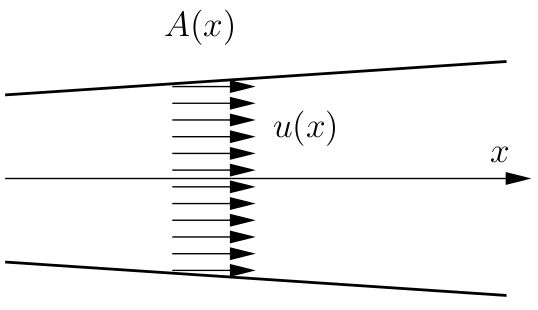
\includegraphics[width=\linewidth]{TeX_files/chapter11-Compresible/conducto1}
			\end{center}
		\end{minipage} & %
		\begin{minipage}[c]{0.6\textwidth}%
			Si derivamos esta ecuación obtenemos 
			
\begin{equation}
				uA\dif\rho+u\rho\dif A+\rho A\dif u=0
\end{equation}
			
			y, dividiendo por $\dot{m}$, 
			
\begin{equation}
				\frac{\dif\rho}{\rho}+\frac{\dif A}{A}+\frac{\dif u}{u}=0
\end{equation}
			
			%
		\end{minipage}\tabularnewline
	\end{tabular}
	
	\medskip{}
	Esto significa que la variación relativa de cualquiera de las tres
	cantidades implica una variación en sentido contrario de, al menos,
	una de las otras dos.

	
	Para ver cómo ocurre esto, consideremos la ecuación de Euler (menospreciamos
	la fricción) para la dirección $x$, estacionaria y sin el término
	de gravedad 
	
\begin{equation}
		u\deriv{u}{x}=-\frac{1}{\rho}\deriv{p}{x}\,\Rightarrow\,\frac{\dif u}{u}=-\frac{\dif p}{\rho u^{2}}
\end{equation}
	
	y, por otro lado, de la expresión de la velocidad del sonido, 
	
\begin{equation}
		\dif p=c^{2}\dif\rho\,\Rightarrow\,\frac{\dif u}{u}=-\frac{c^{2}\dif\rho}{\rho u^{2}}\,\Rightarrow\,\frac{\dif\rho}{\rho}=-\ma^{2}\frac{\dif u}{u}
\end{equation}
	
	
	Introduciendo esto en la ecuación de continuidad, obtenemos 
	
\begin{equation}
		\frac{\dif u}{u}=-\frac{\dif p}{\rho u^{2}}=\frac{1}{\ma^{2}-1}\frac{\dif A}{A}
\end{equation}
	
	\bigskip
	
	\begin{center}
		\begin{tabular}{>{\centering}p{0.2\columnwidth}>{\centering}p{0.05\columnwidth}>{\centering}p{0.2\columnwidth}>{\centering}p{0.2\columnwidth}}
			&  & %
			\noindent\begin{minipage}[c]{1\linewidth}%
				\begin{center}
					\textbf{$\ma<1$}\\
					\textbf{subsónico}
					\par\end{center}%
			\end{minipage} & %
			\noindent\begin{minipage}[c]{1\linewidth}%
				\begin{center}
					\textbf{$\ma>1$}\\
					\textbf{supersónico}
					\par\end{center}%
			\end{minipage}\tabularnewline
			\begin{minipage}[c]{4cm}%
				\begin{center}
					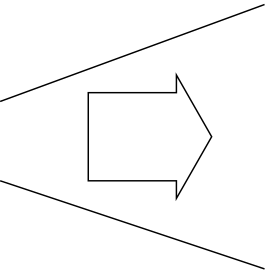
\includegraphics[width=\linewidth]{TeX_files/chapter11-Compresible/conducto2a}
				\end{center}
			\end{minipage} & $A\uparrow$  & %
			\noindent\begin{minipage}[c]{1\linewidth}%
				\begin{center}
					$u\downarrow\,;\,p\uparrow$ \\
					difusor subsónico 
					\par\end{center}%
			\end{minipage} & %
			\noindent\begin{minipage}[c]{1\linewidth}%
				\begin{center}
					$u\uparrow\,;\,p\downarrow$ \\
					inyector supersónico 
					\par\end{center}%
			\end{minipage}\tabularnewline
			\begin{minipage}[c]{4cm}%
				\begin{center}
					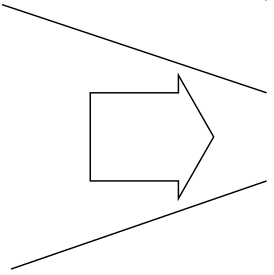
\includegraphics[width=\linewidth]{TeX_files/chapter11-Compresible/conducto2b}
				\end{center}
			\end{minipage} & $A\downarrow$  & %
			\noindent\begin{minipage}[c]{1\linewidth}%
				\begin{center}
					$u\uparrow\,;\,p\downarrow$ \\
					inyector subsónico 
					\par\end{center}%
			\end{minipage} & %
			\noindent\begin{minipage}[c]{1\linewidth}%
				\begin{center}
					$u\downarrow\,;\,p\uparrow$ \\
					difusor supersónico 
					\par\end{center}%
			\end{minipage}\tabularnewline
		\end{tabular}
		\par\end{center}
	
	$\ma=1$ (flujo sónico o crítico) sólo es posible cuando $\dif A=0$,
	es decir, cuando hay un mínimo o un máximo de sección.
	
	En condiciones críticas o sónicas, el flujo másico sigue siendo el
	mismo 
	
\begin{equation}
		\rho^{*}u^{*}A^{*}=\rho uA=\dot{m}\,\Rightarrow\frac{A}{A^{*}}=\frac{\rho^{*}u^{*}}{\rho u},
\end{equation}
	
	que se puede expresar en función de $\gamma$ y $\ma$ (ver Flujo
	Compresible I) 
		\begin{eqnarray*}
			\frac{\rho^{*}}{\rho} & = & \frac{\rho^{*}}{\rho_{0}}\frac{\rho_{0}}{\rho}=\left(\frac{2}{\gamma+1}\right)^{\frac{1}{\gamma-1}}\left(1+\frac{\gamma-1}{2}\ma^{2}\right)^{\frac{1}{\gamma-1}}\\
			\frac{u^{*}}{u} & = & \frac{c^{*}}{u}=\frac{c}{u}\frac{c^{*}}{c}=\frac{1}{\ma}\frac{c^{*}}{c_{0}}\frac{c_{0}}{c}=\frac{1}{\ma}\sqrt{\frac{T^{*}}{T_{0}}}\sqrt{\frac{T_{0}}{T}}=\frac{1}{\ma}\left(\frac{2}{\gamma+1}\right)^{\frac{1}{2}}\left(1+\frac{\gamma-1}{2}\ma^{2}\right)^{\frac{1}{2}}
		\end{eqnarray*}
	
		
\begin{equation}
			\Rightarrow\,\boxed{\frac{A}{A^{*}}=\frac{1}{\ma}\left[\frac{2+(\gamma-1)\ma^{2}}{\gamma+1}\right]^{\frac{1}{2}\frac{(\gamma+1)}{(\gamma-1)}}}
\end{equation}
		
	
	
	Para el caso particular de aire, $\gamma=1.4$, 
	
\begin{equation}
		\frac{A}{A^{*}}=\frac{1}{\ma}\frac{\left(2+0.4\ma^{2}\right)^{3}}{13.824}
\end{equation}
	
	

	
	%\vspace*{-3cm}
	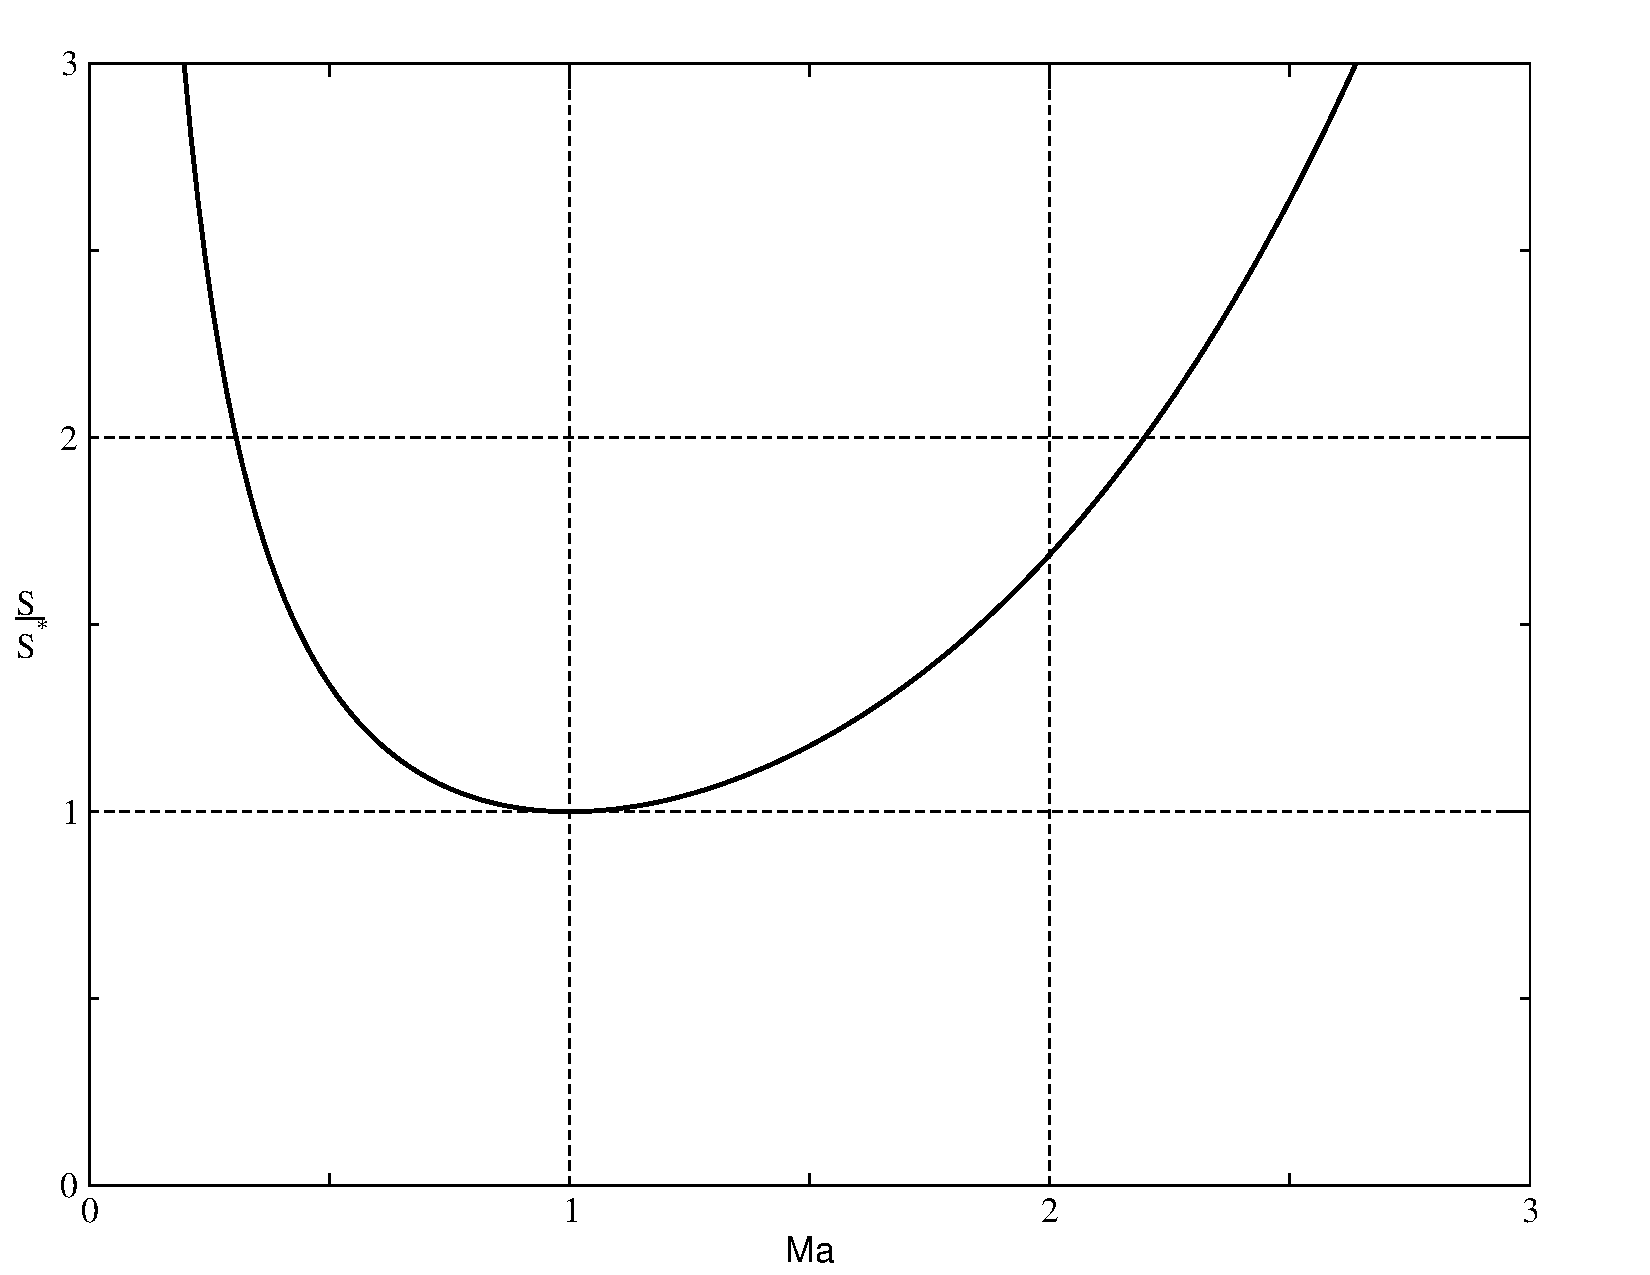
\includegraphics[clip,width=1\linewidth]{TeX_files/chapter11-Compresible/seccion} 
	
	En un flujo isoentrópico en un conducto, las condiciones críticas
	sólo pueden darse en un cuello (área mínima).
	
	Para cualquier valor de $A/A^{*}>1$ hay dos posible soluciones de
	$\ma$, una con $\ma<1$~(flujo subsónico) y otra con $\ma>1$ (flujo
	supersónico).
	\subsection*{Ejemplo :}
		Flujo isoentrópico de aire en un conducto. En la sección 1 las condiciones
		son: 
		\begin{eqnarray*}
			A_{1} & = & 0.05~\text{m}^{2}\\
			u_{1} & = & 180~\text{m/s}\\
			p_{1} & = & 500~\text{kPa}\\
			T_{1} & = & 470~\text{K}
		\end{eqnarray*}
		Calcular $\ma_{1}$, $T_{0}$, $p_{0}$, $A^{*}$ y $\dot{m}$. En
		la sección 2 el área es $A_{2}=0.036~\text{m}^{2}$. Calcular $\ma_{2}$
		y $p_{2}$ suponiendo que el flujo es a)~subsónico y b)~supersónico.

		Calcular la temperatura de estancamiento es fácil, 
		\[
		T_{0}=T_{1}+\frac{u_{1}^{2}}{2c_{p}}=470+\frac{180^{2}}{2\times1005}=486~\text{K}
		\]
		y la velocidad del sonido es 
		\[
		c_{1}=\sqrt{\gamma rT_{1}}=\sqrt{1.4\times287\times470}=435~\text{m/s}
		\]
		y, por lo tanto, 
		\[
		\ma_{1}=\frac{u}{c}=\frac{180}{435}=0.414
		\]
		
		Con $\ma_{1}$ podemos calcular la presión de estancamiento 
		\[
		p_{0}=p_{1}\left(1+0.2\ma_{1}^{2}\right)^{3.5}=500\left(1+0.2\times0.414^{2}\right)^{3.5}=563~\text{kPa}
		\]
		y el área en las condiciones críticas, 
		\[
		\frac{A_{1}}{A^{*}}=\frac{1}{\ma_{1}}\frac{\left(2+0.4\ma_{1}^{2}\right)^{3}}{13.824}=\frac{1}{0.414}\frac{\left(2+0.4\times0.414^{2}\right)^{3}}{13.824}=1.547
		\]
		
		\[
		\Rightarrow\,A^{*}=\frac{A_{1}}{1.547}=\frac{0.05}{1.547}=0.0323~\text{m}^{2}
		\]
		Es completamente imposible tener en el conducto un área menor que
		éste.
		
		Por otro lado, si el flujo ha de pasar a supersónico, sólo es posible
		pasando a través de un estrechamiento con este área.
		
		El flujo másico es 
		\[
		\dot{m}=\rho_{1}u_{1}A_{1}=\frac{p_{1}}{rT_{1}}u_{1}A_{1}=\frac{500\times10^{3}}{287\times170}\times180\times0.05=33.4~\text{kg/s}
		\]

		Si $A_{2}=0.036$, $A_{2}/A^{*}=1.115$. Esto nos ofrece dos posibles
		valores de $\ma_{2}$ 
		\begin{eqnarray*}
			\ma_{2} & = & 0.673\quad\text{(subsónico)}\\
			\ma_{2} & = & 1.400\quad\text{(supersónico)}
		\end{eqnarray*}
		a) En el primer caso, 
		\[
		p_{2}=\frac{p_{0}}{\left[1+0.2\times0.673^{2}\right]^{3.5}}=415.5~\text{kPa}.
		\]
		b) En el segundo caso, 
		\[
		p_{2}=\frac{p_{0}}{\left[1+0.2\times1.400^{2}\right]^{3.5}}=176.9~\text{kPa}.
		\]
		En éste último caso en algún punto anterior a 2 debe haber un cuello
		de área $A^{*}=0.0323~\text{m}^{2}$.


\section{Ondas de choque normales}
	
	En flujo supersónico pueden ocurrir variaciones irreversibles ($\Delta s\neq0$)
	de las propiedades del flujo en un espacio muy pequeño, de forma que
	pueden ser consideradas discontinuidades. Estas discontinuidades se
	conocen como \textcolor{red}{ondas de choque}.
	
	Consideremos que los puntos 1 y 2 son, respectivamente, antes y despues
	de la onda de choque. Para simplificar, vamos a suponer que ésta es
	inmóvil. Procedemos de forma parecida al cálculo de la velocidad del
	sonido.
	
	La ecuación de continuidad debe cumplirse, $\rho_{1}u_{1}=\rho_{2}u_{2}=\text{cte},$
	asi como la conservación de la cantidad de movimiento $p_{1}-p_{2}=\rho_{2}u_{2}^{2}-\rho_{1}u_{1}^{2}$
	y la ecuación de la energía 
\begin{equation}
		h_{1}+\frac{1}{2}u_{1}^{2}=h_{2}+\frac{1}{2}u_{2}^{2}=h_{0}
\end{equation}
	si se considera que no hay fricción.

	
	Eliminando las velocidades de las ecuaciones anteriores, se obtiene
	la \textcolor{blue}{relación de Rankine-Hugoniot} 
	
\begin{equation}
		h_{2}-h_{1}=\frac{1}{2}\left(p_{2}-p_{1}\right)\left(\frac{1}{\rho_{2}}+\frac{1}{\rho_{1}}\right)
\end{equation}
	
	
	\textbf{Actividad 1:} Deducir esta expresión


	Si el gas es perfecto, la entalpía se relaciona con la temperatura,
	la presión y la densidad mediante 
	\[
	h=c_{p}T=\frac{\gamma p}{(\gamma-1)\rho}
	\]
	y tras unas cuantas operaciones, se llega a la relación 
	
\begin{equation}
		\frac{\rho_{2}}{\rho_{1}}=\frac{1+\beta\frac{p_{2}}{p_{1}}}{\beta+\frac{p_{2}}{p_{1}}}\qquad\text{con }\beta=\frac{\gamma+1}{\gamma-1}.
\end{equation}
	
	
	Este proceso no es isoentrópico. Si hubiese sido isoentrópico, la
	relación entre variaciones de presión y de densidad habría sido 
	
\begin{equation}
		\frac{\rho_{2}}{\rho_{1}}=\left(\frac{p_{2}}{p_{1}}\right)^{\frac{1}{\gamma}}
\end{equation}
	
	
	De hecho, se puede calcular la variación de entropía que se produce
	en una onda de choque, suponiendo, como siempre, que el gas es ideal,
	mediante 
	
\begin{equation}		\frac{s_{2}-s_{1}}{c_{v}}=\ln\left[\frac{p_{2}}{p_{1}}\left(\frac{\rho_{1}}{\rho_{2}}\right)^{\gamma}\right]=\ln\left[\frac{p_{2}}{p_{1}}\left(\frac{\beta+\frac{p_{2}}{p_{1}}}{1+\beta\frac{p_{2}}{p_{1}}}\right)^{\gamma}\right]
\end{equation}
	
	
	%\vspace*{-3cm}
	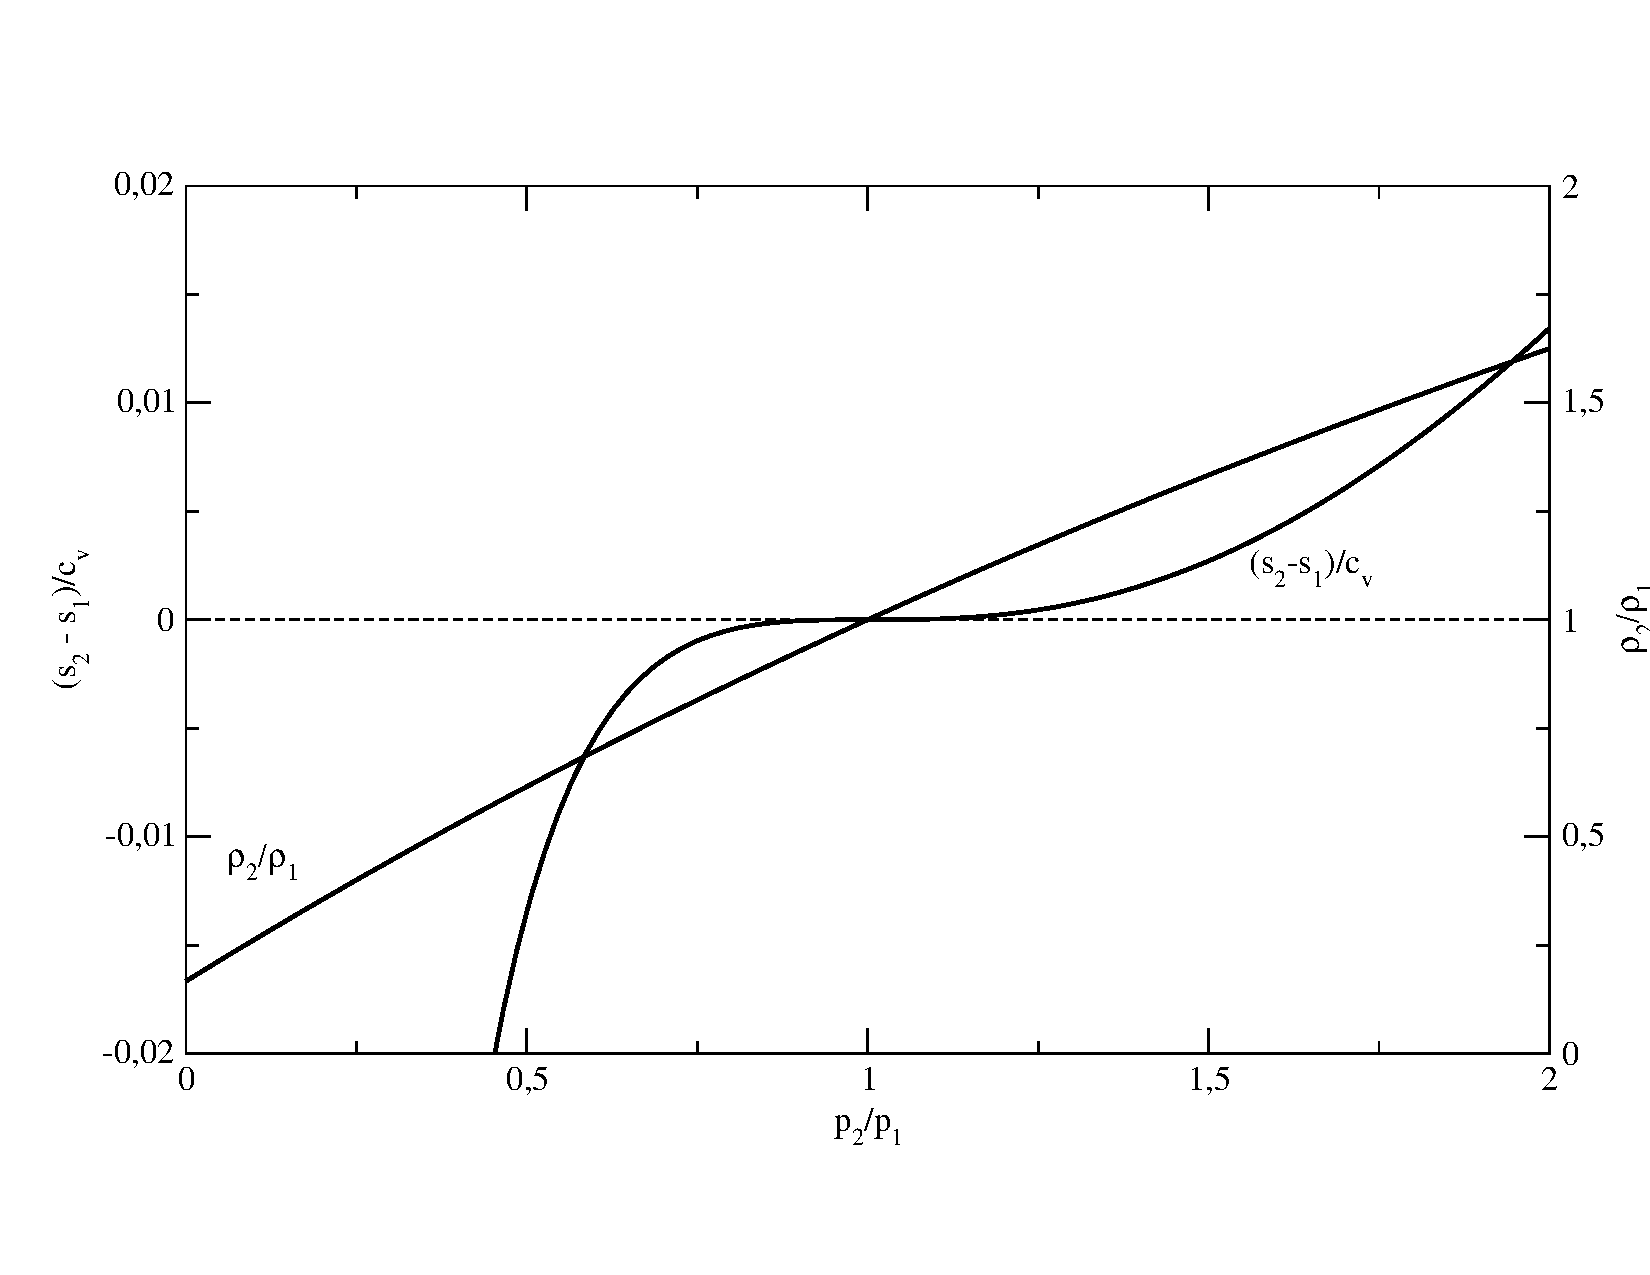
\includegraphics[clip,width=1\linewidth]{TeX_files/chapter11-Compresible/densidades}

	
	De la gráfica anterior se deduce que es imposible una onda de choque
	en la que $p_{2}<p_{1}$ (rarefacción), ya que esto implicaría una
	disminución de la entropía.
	
	En general, las ondas de choque son procesos, aunque adiabáticos,
	no isoentrópicos. Sólo para ondas muy débiles ($p_{2}\approx p_{1}$)
	se pueden considerar isoentrópicos.
	
	Dado que para un gas perfecto, la relación entre presión dinámica
	y presión estática se puede expresar de foma adimensional en función
	de $\gamma$ y el número de Mach, 
	
\begin{equation}
		\frac{\rho u^{2}}{p}=\frac{u^{2}}{rT}=\frac{\gamma u^{2}}{\gamma rT}=\frac{\gamma u^{2}}{c^{2}}=\gamma\ma^{2},
\end{equation}
	
	es posible expresar la relación de presiones antes y después de la
	onda de choque en función de $\gamma$ y el número de Mach en 1, 
	
\begin{equation}		\frac{p_{2}}{p_{1}}=\frac{2\gamma\ma_{1}^{2}-(\gamma-1)}{\gamma+1}.
\end{equation}
	
	

	
	Es importante observar que, para cualquier valor de $\gamma$, si
	debemos tener $\frac{p_{2}}{p_{1}}>1$ de forma que el proceso sea
	real, \textcolor{red}{debe cumplirse que $\ma_{1}>1$}.
	
	Por otro lado, es posible deducir una expresión que relacione el número
	de Mach antes y después de la onda de choque, 
	
\begin{equation}
	\ma_{2}^{2}=\frac{{\gamma-1}\ma_{1}^{2}+2}{2\gamma\ma_{1}^{2}-(\gamma-1)}
\end{equation}
	
	
	\textbf{Actividad 2:} Deducir esta expresión y la anterior.

	En esta última expresión, para $\ma_{1}>1$, el denominador siempre
	es mayor que el numerador, de forma, que $\ma_{2}<1$

	
	En conclusión, una onda de choque, es una transición, casi singular,
	\textcolor{red}{siempre de flujo supersónico a flujo subsónico}. Además,
	el proceso \textcolor{red}{no es isoentrópico} y \textcolor{red}{la
		presión después es mayor que antes} de la onda. 

	\textbf{Actividad 3:} Deducir las relaciones
		
		
\begin{equation}			\frac{\rho_{2}}{\rho_{1}}=\frac{u_{1}}{u_{2}}=\frac{\left(\gamma+1\right)\ma_{1}^{2}}{\left(\gamma-1\right)\ma_{1}^{2}+2}
\end{equation}
		
		
		
		\begin{equation}
			\frac{T_{2}}{T_{1}}=\left[2+\left(\gamma-1\right)\ma_{1}^{2}\right]\frac{2\gamma\ma_{1}^{2}-\left(\gamma-1\right)}{\left(\gamma+1\right)^{2}\ma_{1}^{2}}
		\end{equation}
		
		
		
		\begin{equation}
			\frac{p_{02}}{p_{01}}=\frac{\rho_{02}}{\rho_{01}}=\left[\frac{\left(\gamma+1\right)\ma_{1}^{2}}{2+\left(\gamma-1\right)\ma_{1}^{2}}\right]^{\frac{\gamma}{\gamma-1}}\left[\frac{\gamma+1}{2\gamma\ma_{1}^{2}-\left(\gamma-1\right)}\right]^{\frac{1}{\gamma-1}}
		\end{equation}
		
\section{Toberas}

\subsection{Tobera convergente}

\begin{center}
	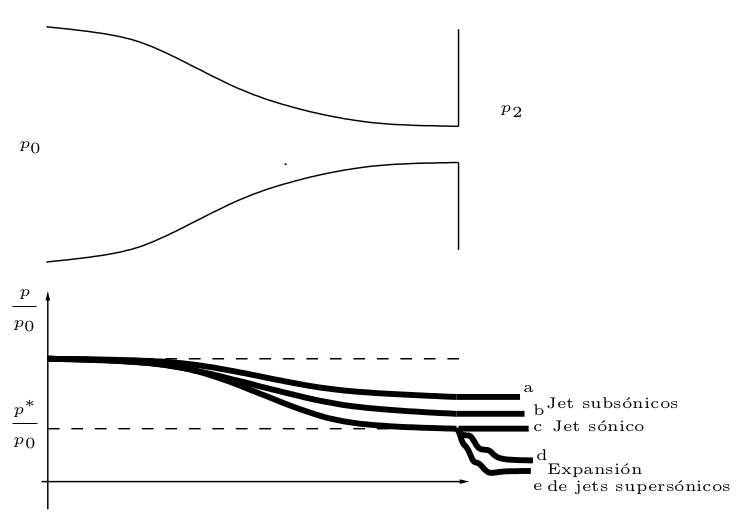
\includegraphics[width=0.7\linewidth]{TeX_files/chapter11-Compresible/tobera_convergente}
\end{center}


	Como vimos en anteriormente, el flujo másico se puede calcular
	como
	\[
	\dot{m}=\rho^{*}u^{*}S^{*}
	\]
	
	Por otro lado, las propiedades críticas son función únicamente de
	las propiedades totales, y $\gamma$. Las recordamos:
	\[
	\begin{array}{cc}
		p^{*}=p_{0}\left(\frac{2}{\gamma+1}\right)^{\frac{\gamma}{\gamma-1}}; & T^{*}=T_{0}\frac{2}{\gamma+1}\\
		\rho^{*}=\rho_{0}\left(\frac{2}{\gamma+1}\right)^{\frac{1}{\gamma-1}}; & c^{*}=c_{0}\left(\frac{2}{\gamma+1}\right)^{\frac{1}{2}}(=u^{*})
	\end{array}
	\]
	
	Por lo tanto, si las propiedades totales (aguas arriba) no cambian,
	el flujo másico tampoco, independientemente de las condiciones aguas
	abajo (en la salida). Se dice entonces que el flujo está \textbf{bloqueado}.

	
	La interpretación física es que si el flujo es supersónico, su velocidad
	es mayor que la cualquier perturbación (es decir, información) que
	se pueda trasmitir a través del medio. Y por lo tanto, la información
	que se transmite hacia atrás (aguas arriba) nunca llega a destino.
	Es decir, que el fluido que se encuentra en la sección crítica no
	tiene forma de saber qué condiciones hay aguas abajo y éstas no le
	pueden afectar.
	
	\begin{center}
		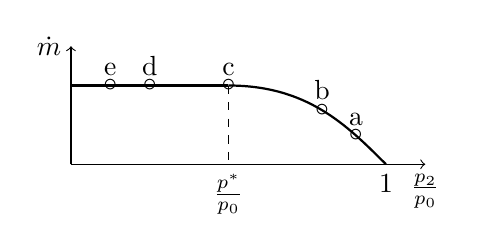
\begin{tikzpicture}
			\draw[->](0,0)--(4.5,0) node[anchor=north]{$\frac{p_2}{p_0}$};
			\draw[->](0,0)--(0,1.5) node[anchor=east]{$\dot{m}$};
			\draw[thick](0,1)--
			node[near start]{$\circ$}
			node[near start,above]{e}
			node[midway]{$\circ$}
			node[midway,above]{d}
			(2,1)
			node{$\circ$}
			node[above]{c};
			\draw[thick](2,1) ..controls (3,1) and (3.5,0.5).. 
			node[midway]{$\circ$}
			node[midway,above]{b}
			node[near end]{$\circ$}
			node[near end,above]{a}
			(4,0)
			node[below]{1};
			\draw[dashed](2,1)--(2,0)
			node[below]{$\frac{p^*}{p_0}$};
		\end{tikzpicture}
		\par\end{center}
	


\subsection{Tobera convergente-divergente}

\begin{center}
	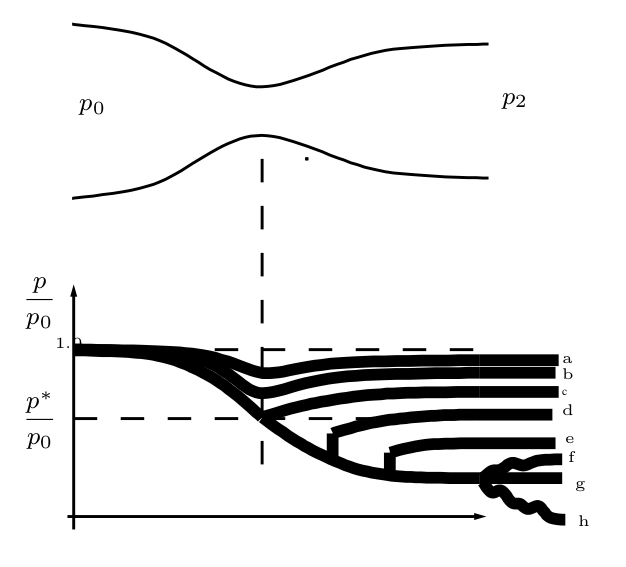
\includegraphics[width=0.7\linewidth]{TeX_files/chapter11-Compresible/tobera_convergente_divergente}
\end{center}

	
	Si el flujo es supersónico (está bloqueado) pero las condiciones en
	la salida no son las adecuadas para mantenerlo en este estado, el
	flujo salta de forma irreversible, con una onda de choque, a un estado
	subsónico que le permita llegar al exterior con las condiciones.
	
	Las condiciones para la que el flujo se mantiene supersónico sin crear
	una onda de choque (caso $g$) se dicen que son las \emph{condiciones
		de diseño de la tobera}.
	
	\begin{center}
		\begin{tikzpicture}
			\draw[->](0,0)--(4.5,0) node[anchor=north]{$\frac{p_2}{p_0}$};
			\draw[->](0,0)--(0,1.5) node[anchor=east]{$\dot{m}$};
			\draw[thick](0,1)--
			node[very near start]{$\circ$}
			node[very near start,above]{h}
			node[near start]{$\circ$}
			node[near start,above]{g}
			node[midway]{$\circ$}
			node[midway,above]{f}
			node[near end]{$\circ$}
			node[near end,above]{e}
			node[very near end]{$\circ$}
			node[very near end,above]{d}
			(2,1)
			node{$\circ$}
			node[above]{c};
			\draw[thick](2,1) ..controls (3,1) and (3.5,0.5).. 
			node[midway]{$\circ$}
			node[midway,above]{b}
			node[near end]{$\circ$}
			node[near end,above]{a}
			(4,0)
			node[below]{1};
			\draw[dashed](2,1)--(2,0)
			node[below]{$\binom{\frac{p^*}{p_0}}{\textrm{\tiny{(en la garganta)}}}$};
		\end{tikzpicture}
		\par\end{center}
	
	
	Si la presión en la descarga ($p_{2}$) es inferior a la presión de
	diseño de la tobera ($p^{*}$para la tobera convergente y $p_{g}$
	para la convergente-divergente) el flujo no puede bajar su presión
	mediante ondas de choque, ya que esto implicaría una disminución de
	la entropía. El flujo se expande en este caso mediante una \emph{expansión
		de Prandtl-Meyer}. Es una compleja expansión supersónica isentrópica
	en forma de abanico, en la que $\ma$ aumenta, y la presión disminuye.

	
	\textbf{Ejemplo:}
		En un tanque hay aire con una presión de $\unit[300]{kPa}$y una
		temperatura de $\unit[20]{^{\circ}C}$. A través de un conducto convergente,
		con un diámetro final de $\unit[4]{cm}$, se descarga el aire en otro
		tanque en el que la presión es de $\unit[200]{kPa}$. Considerando
		$\gamma=1.4$, queremos calcular el flujo másico.
		
		La presión para la cual obtendríamos flujo sónico y, por lo tanto
		bloqueado, es
		\[
		p^{*}=p_{0}\left(\frac{2}{\gamma+1}\right)^{\frac{\gamma}{\gamma-1}}=0.5283p_{0}=\unit[158.48]{kPa}
		\]
		
		La presión que tenemos en la salida es mayor, por lo que el flujo
		no se bloquea.

		El flujo másico lo calculamos mediante las condiciones en la salida,
		suponiendo flujo isentrópico,{\footnotesize{}
			\[
			\dot{m}=\rho_{2}u_{2}S_{2}=p_{2}\sqrt{\frac{\gamma}{rT_{2}}}\ma_{2}S_{2}=p_{0}\sqrt{\frac{\gamma}{rT_{0}}}\ma_{2}S_{2}\left[1+\frac{\gamma-1}{2}\ma^{2}\right]^{\frac{\gamma+1}{2\left(1-\gamma\right)}}
			\]
		}{\footnotesize\par}
		
		Para calcular el número de Mach en la salida
		\[
		\frac{p_{0}}{p_{2}}=\left[1+\frac{\gamma-1}{2}\ma_{2}^{2}\right]^{\frac{\gamma}{\gamma-1}}\;\Rightarrow\;\ma_{2}=0.784
		\]
		
		y el flujo es entonces $\unitfrac[0.852]{kg}{s}$.
		
		Si la presión en el recipiente de descarga estuviese por debajo de
		$\unit[158.48]{kPa}$, el flujo másico sería máximo,
		
		{\footnotesize{}
			\[
			\dot{m}_{\textrm{max}}=\rho^{*}u^{*}S^{*}=p^{*}\sqrt{\frac{\gamma}{rT^{*}}}S^{*}=p_{0}\sqrt{\frac{\gamma}{rT_{0}}}S_{2}\left[\frac{\gamma+1}{2}\right]^{\frac{\gamma+1}{2\left(1-\gamma\right)}}=\unitfrac[0.890]{kg}{s}
			\]
		}{\footnotesize\par}
		
		y es independiente del valor de $p_{2}$.


\section{El cono de Mach}

	
	\begin{center}
		\begin{animateinline}[poster=last,controls]{8}
			\multiframe{80}{rt=0+0.05,rv=0+0,rc=1+0,rperiod=0.2+0}{
				\begin{tikzpicture}[>=stealth]
					\clip (-6,-3) rectangle (0.5,3);
					\draw(-7,0) -- (1,0);
					\node at (-2.5,-2.5) {Ma=0};
					\fill[black](-\rv*\rt,0) circle (0.05);
					\foreach \w in {0,1,...,19}{
						\pgfmathparse{max(\rc*\rt-\rc*\rperiod*\w,0)}
						\let\radius\pgfmathresult
						\draw (-\rv*\rperiod*\w,0) circle(\radius);
						}
				\end{tikzpicture}
			}
			
		\end{animateinline}
		\par\end{center}
	

	
	\begin{center}
		\begin{animateinline}[poster=last,controls]{8}
			\multiframe{80}{rt=0+0.05,rv=0.5+0,rc=1+0,rperiod=0.2+0}{
				\begin{tikzpicture}[>=stealth]
					\clip (-6,-3) rectangle (0.5,3);
					\draw(-7,0) -- (1,0);
					\node at (-2.5,-2.5) {Ma=0.5};
					\fill[black](-\rv*\rt,0) circle (0.05);
					\foreach \w in {0,1,...,19}{
						\pgfmathparse{max(\rc*\rt-\rc*\rperiod*\w,0)}
						\let\radius\pgfmathresult
						\draw (-\rv*\rperiod*\w,0) circle(\radius);
						
					}
				\end{tikzpicture}
			}
			
		\end{animateinline}
		\par\end{center}
	

	
	\begin{center}
		\begin{animateinline}[poster=last,controls]{8}
			\multiframe{80}{rt=0+0.05,rv=1+0,rc=1+0,rperiod=0.2+0}{
				\begin{tikzpicture}[>=stealth]
					\clip (-6,-3) rectangle (0.5,3);
					\draw(-7,0) -- (1,0);
					\node at (-2.5,-2.5) {Ma=1};
					\fill[black](-\rv*\rt,0) circle (0.05);
					\foreach \w in {0,1,...,19}{
						\pgfmathparse{max(\rc*\rt-\rc*\rperiod*\w,0)}
						\let\radius\pgfmathresult
						\draw (-\rv*\rperiod*\w,0) circle(\radius);
						
					}
				\end{tikzpicture}
			}
			
		\end{animateinline}
		\par\end{center}
	

	
	\begin{center}
		\begin{animateinline}[poster=last,controls]{8}
			\multiframe{80}{rt=0+0.05,rv=2.5+0,rc=1+0,rperiod=0.2+0}{
				\begin{tikzpicture}[>=stealth]
					\clip (-6,-3) rectangle (0.5,3);
					\draw(-7,0) -- (1,0);
					\node at (-2.5,-2.5) {Ma=2.5};
					\fill[black](-\rv*\rt,0) circle (0.05);
					\foreach \w in {0,1,...,19}{
						\pgfmathparse{max(\rc*\rt-\rc*\rperiod*\w,0)}
						\let\radius\pgfmathresult
						\draw (-\rv*\rperiod*\w,0) circle(\radius);
						
					}
				\end{tikzpicture}
			}
			
		\end{animateinline}
		\par\end{center}
	
	
	En la figura, tomada del White\cite{White2008}, una fuente sonora
	se mueve con una velocidad $U$, que puede ser menor, igual o mayor
	que la velocidad del sonido (en la figura, denominada $a$)
	
	\begin{center}
		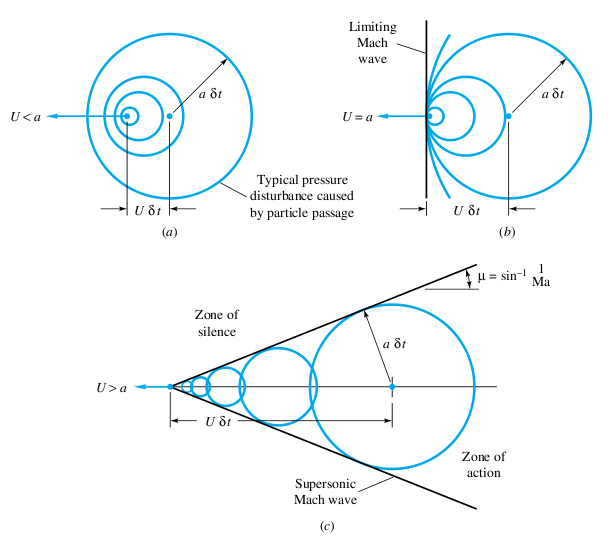
\includegraphics[height=5cm]{TeX_files/chapter11-Compresible/cono_de_Mach}
		\par\end{center}
	
	
	Si la velocidad del objeto es mayor que la del sonido, se forma el
	denominado \emph{cono de Mach }(hay que considerar que es tridimensional).
	Lo que hay fuera del cono en un cierto instante es la zona de silencio.
	Un objeto en esta zona no es capaz de ``oir'' la fuente de sonido
	hasta que la onda de Mach no le alcance.
	\textbf{Actividad 1:}
		Un micrófono está situado en la cima de una colina, y ``oye''
		un objeto supersónico cuando éste se encuentra a 500 m en horizontal
		de su posición. Sabiendo que el objeto vuela a 850 m/s y que la temperatura
		ambiente es de 288 K, calcular la altura a la que vuela el objeto
		por encima del micrófono.


\section{Onda de choque oblicua}

	
	En ocasiones un flujo supersónico es desviado por un objeto. Se crea
	entonces una onda de choque oblicua que forma un ángulo $\beta$ con
	el flujo, que es más o menos arbitrario. El flujo es entonces deflectado
	un ángulo $\theta$ que es función de $\beta$ y de las condiciones
	aguas arriba. 
	
	El flujo antes de la onda de choque es supersónico. Después puede
	ser subsónico, sónico o supersónico, dependiendo de las condiciones.
	
	Aplicando la conservación de masa, cantidad de movimiento y energía
	en un VC que encierra únicamente un área $S$ de la onda de choque,
	obtenemos
	
	\[
	\begin{array}{cc}
		\rho_{1}u_{n1}=\rho_{2}u_{n2} & p_{1}-p_{2}=\rho_{2}u_{n2}^{2}-\rho_{1}u_{n1}^{2}\\
		h_{0}=h_{1}+\frac{1}{2}u_{1}^{2}=h_{2}+\frac{1}{2}u_{2}^{2} & 0=\rho_{1}u_{n1}(u_{t2}-u_{t1})
	\end{array}
	\]
	
	
	\begin{center}
		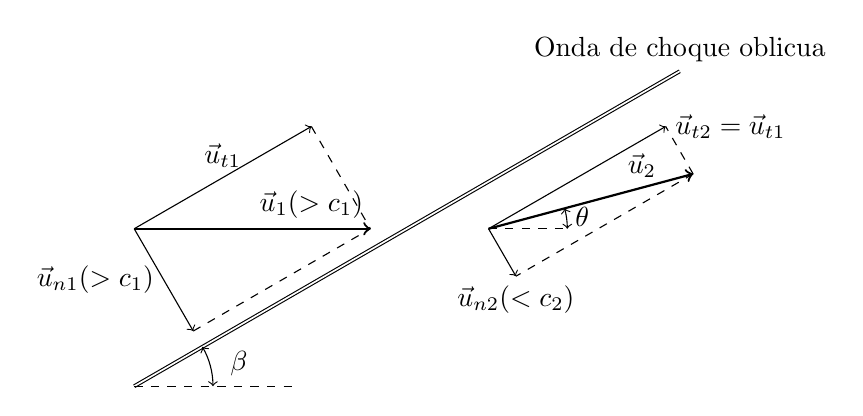
\begin{tikzpicture}
			\draw[double](0,0)--(30:8) node[above]{Onda de choque oblicua};
			\draw[thick,->](0,2) -- node[near end,above]{$\vec{u}_1(>c_1)$} (3,2) ;
			\draw[->](0,2)-- node[midway,left]{$\vec{u}_{n1}(>c_1)$} +(-60:1.5);
			\draw[->](0,2)-- node[midway,above]{$\vec{u}_{t1}$} +(30:2.598);
			\draw[dashed](0,2)++(30:2.598)--(3,2);
			\draw[dashed](0,2)++(-60:1.5)--(3,2);
			\draw[dashed](0,0)--(2,0);
			\draw[<->](1,0)  arc (0:30:1) ;
			\draw(15:1.1) node[right=1pt]{$\beta$};
			%
			\draw[thick,->](4.5,2)-- node[near end,above]{$\vec{u}_2$} +(15:2.690);
			\draw[->](4.5,2)--  +(30:2.598) node[right]{$\vec{u}_{t2}=\vec{u}_{t1}$};
			\draw[->](4.5,2)--  +(-60:0.696) node[below]{$\vec{u}_{n2}(<c_2)$};
			\draw[dashed](4.5,2)+(15:2.690)--+(-60:0.696);
			\draw[dashed](4.5,2)+(15:2.690)--+(30:2.598);
			\draw[dashed](4.5,2)--+(0:1);
			\draw[<->](4.5,2)+(0:1) arc(0:15:1);
			\draw(4.5,2)+(7.5:1.2) node{$\theta$};
		\end{tikzpicture}
		\par\end{center}
	
	
	La única diferencia entre estas ecuaciones y las relativas a la onda
	de choque normal es que se añade una velocidad tangencial, que és
	idéntica a ambos lados de la onda, $u_{t1}=u_{t2}=u_{t}$, y cuyo
	único efecto es aumentar en $\frac{1}{2}u_{t}^{2}$ la energía.
	
	Por lo demás són idénticas, con las velocidades normales $u_{n1}$
	y $u_{n2}$ en los papeles de velocidades en la onda de choque normal. 
	
	Lo único que hay que hacer es definir un \emph{número de Mach normal},
	
\begin{equation}
		\ma_{n}=\frac{u_{n}}{c}
\end{equation}
	
	
	y las relaciones que obtuvimos para ondas de choque normales se escriben
	ahora como
	
\begin{equation}		\frac{p_{2}}{p_{1}}=\frac{2\gamma\ma_{n1}^{2}-(\gamma-1)}{\gamma+1}
\end{equation}
	
	
	
	\begin{equation}
		\ma_{n2}^{2}=\frac{\left(\gamma-1\right)\ma_{n1}^{2}+2}{2\gamma\ma_{n1}^{2}-(\gamma-1)}
	\end{equation}
	
	

	
	
	\begin{equation}
		\frac{\rho_{2}}{\rho_{1}}=\frac{u_{n1}}{u_{n2}}=\frac{\left(\gamma+1\right)\ma_{n1}^{2}}{\left(\gamma-1\right)\ma_{n1}^{2}+2}=\frac{\tan\beta}{\tan\left(\beta-\theta\right)}
	\end{equation}
	
	
	
	\begin{equation}
		\frac{T_{2}}{T_{1}}=\left[2+\left(\gamma-1\right)\ma_{n1}^{2}\right]\frac{2\gamma\ma_{n1}^{2}-\left(\gamma-1\right)}{\left(\gamma+1\right)^{2}\ma_{n1}^{2}}
	\end{equation}
	
	
	
	\begin{equation}
		\frac{p_{02}}{p_{01}}=\frac{\rho_{02}}{\rho_{01}}=\left[\frac{\left(\gamma+1\right)^{2}\ma_{n1}^{2}}{2+\left(\gamma-1\right)\ma_{n1}^{2}}\right]^{\frac{\gamma}{\gamma-1}}\left[\frac{\gamma+1}{2\gamma\ma_{n1}^{2}-\left(\gamma-1\right)}\right]^{\frac{1}{\gamma-1}}
	\end{equation}
	
	
	En la siguiente gráfica se ha representado $\ma_{n1}$ en función
	de $\beta$ para diferentes valores de $\theta$, usando la primera
	de las expresiones dadas. 

	
	\begin{center}
		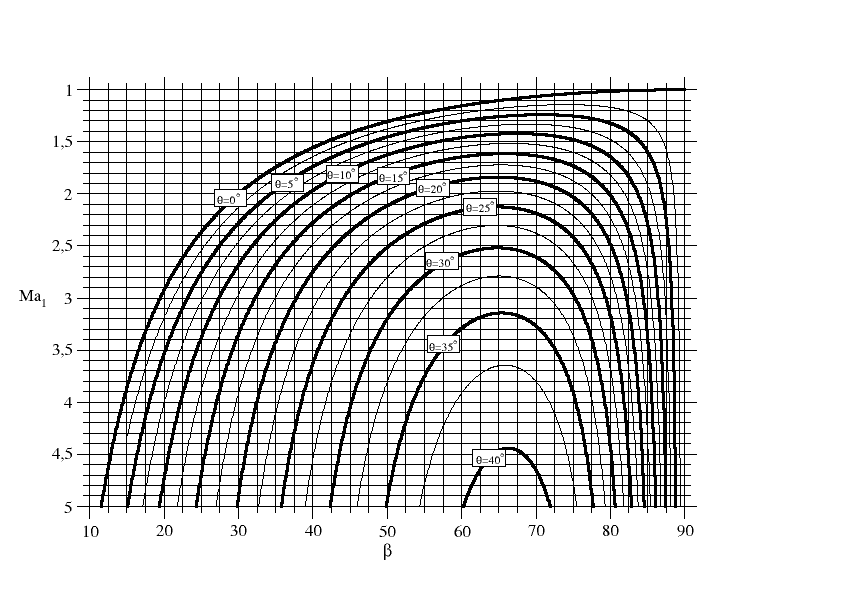
\includegraphics[width=0.7\textwidth]{TeX_files/chapter11-Compresible/oblicuas}
		\par\end{center}
	
	
	Calculemos el ángulo de deflección $\theta$. De la figura de la onda
	de choque oblicua se puede deducir por trigonometría que 
	
	
\begin{equation}
		\theta=\arctan\frac{u_{t}}{u_{n2}}-\arctan\frac{u_{t}}{u_{n1}}
\end{equation}
	
	
	Podemos ahora calcular el valor de $u_{t}$ para el cuál el ángulo
	de deflección en máximo,
	
	\begin{equation}
		\frac{\dif\theta}{\dif u_{t}}=0\;\Rightarrow\;\frac{u_{t}}{u_{n1}}=\sqrt{\frac{u_{n2}}{u_{n1}}};\frac{u_{t}}{u_{n2}}=\sqrt{\frac{u_{n1}}{u_{n2}}}
	\end{equation}
	
	
	
	\begin{equation}
		\Rightarrow\;\theta_{\textrm{max}}=\arctan\sqrt{\frac{u_{n1}}{u_{n2}}}-\arctan\sqrt{\frac{u_{n2}}{u_{n1}}}
	\end{equation}
	
	
	Esto limita bastante los posibles valores de deflección
	\textbf{Ejemplo:}
		Para $\ma_{n1}=5.0$ y $\gamma=1.4$, se tiene $\frac{u_{n1}}{u_{n2}}=5$
		y el ángulo de deflección máxima es $\theta_{\textrm{max}}=41.81^{\circ}$


	
	\textbf{Actividad 2:} Calcular el ángulo de deflección máximo para un flujo incidente con
		$\ma_{n1}\rightarrow\infty$.

	Para una $\vec{u}_{1}$, $c_{1}$ y $\gamma$ dadas, es posible resolver
	las ecuaciones para encontrar todos los valores posibles de $\vec{u}_{2}=u_{2x}\vec{\imath}+u_{2y}\vec{\jmath}$.
	El resultado es una \emph{hodografía.}
	
	\begin{center}
		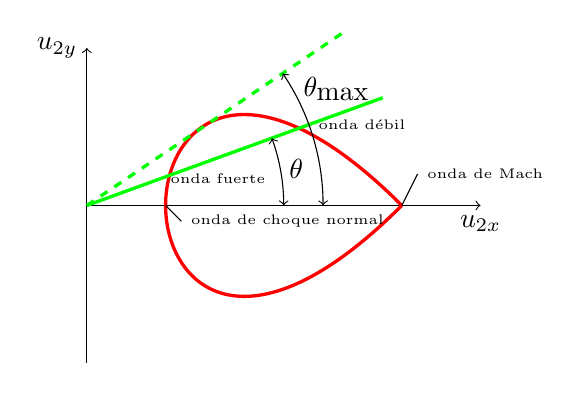
\begin{tikzpicture}
			\draw[->](0,0)--(5,0) node[below]{$u_{2x}$};
			\draw[->](0,-2)--(0,2) node[left]{$u_{2y}$};
			\draw[color=red,very thick] (4,0) ..controls (2,2) and (1,1) ..(1,0);
			\draw[color=red,very thick] (4,0) ..controls (2,-2) and (1,-1) ..(1,0);
			\draw[color=green,very thick] (0,0) -- (20:4);
			\draw(0,0)+(20:1) node[right]{\tiny onda fuerte};
			\draw(0,0)+(20:3) node[right]{\tiny onda débil};
			\draw[color=green,very thick,dashed] (0,0) -- (34:4);
			\draw[<->](2.5,0)arc(0:20:2.5);
			\draw(0,0)+(10:2.7) node{$\theta$};
			\draw[<->](3,0)arc(0:34:3);
			\draw(0,0)+(25:3.5) node{$\theta_{\textrm{max}}$};
			\draw(4,0)--(4.2,0.4) node[right]{\tiny onda de Mach};
			\draw(1,0)--(1.2,-0.2) node[right]{\tiny onda de choque normal};
		\end{tikzpicture}
		\par\end{center}
	

